
\documentclass[conference]{IEEEtran}
\IEEEoverridecommandlockouts
% The preceding line is only needed to identify funding in the first footnote. If that is unneeded, please comment it out.
\usepackage{cite}
\usepackage{amsmath,amssymb,amsfonts}
\usepackage{algorithmic}
\usepackage{graphicx}
\usepackage{array}
\usepackage{textcomp}
\usepackage{xcolor}
\usepackage{fixltx2e}
\usepackage{enumitem}
\def\BibTeX{{\rm B\kern-.05em{\sc i\kern-.025em b}\kern-.08em
    T\kern-.1667em\lower.7ex\hbox{E}\kern-.125emX}}
\begin{document}

\title{Filter design using Convex Optimization}

\author{\IEEEauthorblockN{Satheesh Kumar Simhachalam}
\IEEEauthorblockA{\textit{EE22RESCH11010}
}
\and
\IEEEauthorblockN{Parv Chandola}
\IEEEauthorblockA{\textit{EE22MTECH12005} \\
}
}

\maketitle

\section{Introduction}
Filter design is an important task in signal processing, which involves designing a system that can selectively pass or reject certain frequency components of a signal. Convex optimization is a mathematical technique that can be used to solve many engineering problems, including filter design.

Convex optimization provides a rigorous and efficient framework for solving many optimization problems, including those arising in filter design. It ensures that the designed filter has desirable properties such as stability, causality, and minimum phase, which are important for practical applications.

Moreover, convex optimization allows the designer to specify the desired frequency response of the filter in a flexible and accurate manner. This is achieved by formulating the filter design problem as an optimization problem with convex constraints and objectives. The convexity of the optimization problem guarantees that it can be efficiently solved using numerical algorithms, and that the solution is globally optimal.

In summary, the need to do filter designing using convex optimization arises from the desire to obtain a filter with desirable properties and a flexible and accurate frequency response, while ensuring efficient and reliable design.

\section{FIR Filters}
\subsection{Definition}
In signal processing, a finite impulse response (FIR) filter is a filter whose impulse response (or response to any finite length input) is of finite duration, because it settles to zero in finite time. This is in contrast to infinite impulse response (IIR) filters, which may have internal feedback and may continue to respond indefinitely (usually decaying).

The impulse response of an Nth-order discrete-time FIR filter (i.e., with a Kronecker delta impulse input) lasts for N + 1 samples, and then settles to zero.

FIR filters can be discrete-time or continuous-time, and digital or analog
\begin{figure}[!h]
	\begin{center} 
	    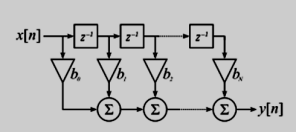
\includegraphics[width=0.8\columnwidth]{figs/FIR}
	\end{center}
\caption{FIR filter block diagram}
\label{fig:Fig1}
\end{figure}

A discrete-time FIR filter of order $N$. The top part is an $N$-stage delay line with $N+1$ taps. Each unit delay is a $z^-1$ operator in the Z-transform notation. The output $y$ of a linear time invariant system is determined by convolving its input signal $x$ with its impulse response $a$. For a discrete-time FIR filter, the output is a weighted sum of the current and a finite number of previous values of the input. The operation is described by the following equation, which defines the output sequence $y[n]$ in terms of input sequence $x[n]$.
\begin{align}
y[n] &= a_0x[n]+a_1x[n-1]+---+a_Nx[n-N]\\
 	 &= \sum_{i=0}^{N}a_ix[n-i] 
\end{align} 
where,
\begin{itemize}
\item $x[n]$ is the input signal
\item $y[n]$ is the output signal
\item $a_i$ are the filter coefficients, also known as tap weights, that make up the impulse response
\item $N$ is the filter order
\end{itemize}

\subsection{FIR properties}
An FIR filter has a number of useful properties which sometimes make it preferable to an infinite impulse response (IIR) filter. FIR filters:
\begin{itemize}
\item\textbf{Require no feedback} This means that any rounding errors are not compounded by summed iterations. The same relative error occurs in each calculation. This also makes implementation simpler.
\item\textbf{Inherent stability} This is due to the fact that, because there is no required feedback, all
the poles are located at the origin and thus are located within the unit circle (the required condition for stability in a Z transformed system).
\item\textbf{Phase issue} can easily be designed to be linear phase by making the coefficient sequence symmetric; linear phase, or phase change proportional to frequency, corresponds to equal delay at all frequencies. This property is sometimes desired for phase-sensitive applications, for example data communications, crossover filters, and mastering.

The main disadvantage of FIR filters is that considerably more computation power in a general purpose processor is required compared to an IIR filter with similar sharpness or selectivity, especially when low frequency (relative to the sample rate) cutoffs are needed. However many digital signal processors provide specialized hardware features to make FIR filters approximately as efficient as IIR for many applications.
\end{itemize}

\subsection{FIR Impulse response}
The impulse response $h[n]$ can be calculated if we set $x[n] = \delta[n]$ in the above relation, where $\delta[n]$ is the Kronecker delta impulse. The impulse response for an FIR filter then becomes the set of coefficients $a_n$, as follows
\begin{align}
h[n] = \sum_{i=0}^{N}a_i\delta[n-i] = a_n
\end{align}
The Z-transform of the impulse response yields the transfer function of the FIR filter
\begin{align}
H(z) &= Z(h[n])\\
	 &= \sum_{n=-\infty}^{\infty}h[n]z^{-n}\\
	 &= \sum_{n=0}^{N}a_nz^{-n}
\end{align}\\
\section{FIR Low pass filter design}
Considering the (symmetric, linear phase) finite impulse response(FIR) filter described by its frequency response
\begin{align}
H(\omega) = a_0 + \sum_{k=1}^{N}a_kcosk\omega
\end{align}
where $\omega \in [0,\pi]$ is the frequency. The design variables in our problem are the real coefficients $a = (a_0,....,a_N)\in \textbf{R}^{N+1}$, where N is called the order or length of the FIR filter. In this problem we will explore the design of a low-pass filter, with specifications:
\begin{itemize}
\item For $0\le\omega\le\pi/3,0.89\le H(\omega)\le1.12$,i.e., the filter has about $\pm$1dB ripple in the passband $[0,\pi/3]$.
\item For $\omega_c\le\omega\le\pi, |H(\omega)|\le \alpha$. In other words, the filter achieves an attenuation given by $\alpha$ in the stopband $[\omega_c,\pi]$. Here $\omega_c$ is called the filter cutoff frequency.
\end{itemize} 
\subsection{Problem formulation}
\begin{enumerate}[label=(\alph*)]
\item \textit{Maximum stopband attenuation.} We fix $w_c$ and $N$, and wish to maximize the stopband attenuation, i.e., minimize $\alpha$.

The problem can be expressed as
\begin{align}
\text{minimize } \alpha\\
\text{subject to } f_1(a)&\le 1.12\\
				   f_2(a)&\ge 0.89\\
				   f_3(a)&\le \alpha\\
				   f_4(a)&\ge -\alpha
\end{align}
where,
\begin{align}
f_1(a) &= \underset{0\le \omega \le pi/3}{\text{sup}}H(\omega)\\
f_2(a) &= \underset{0\le \omega \le pi/3}{\text{inf}}H(\omega)\\
f_3(a) &= \underset{0\le \omega \le pi}{\text{sup}}H(\omega)\\
f_4(a) &= \underset{0\le \omega \le pi}{\text{inf}}H(\omega)
\end{align}
for each $\omega$, $H(\omega)$ is a linear function of $a$. Hence the functions $f_1$ and $f_3$ are convex, and $f_2$ and $f_4$ are concave. It follows that the problem is convex.

\item \textit{Minimum transition band}. We fix $N$ and $\alpha$, and want to minimize $\omega_c$, i.e., we set the stopband attenuation and filter length, and wish to minimize the transition band (between $\pi/3$ and $\omega_c$).
This problem can be expressed as
\begin{align}
\text{minimize } f_5(a)\\
\text{subject to } f_1(a)&\le 1.12\\
				   f_2(a)&\ge 0.89\\
\end{align}
where $f_1$ and $f_2$ are the same functions as above, and
\begin{align}
f_5(a) &= inf\{\Omega| -\alpha\le H(\omega)\le \alpha \text{ for } \Omega \le \omega \le \pi\}
\end{align}
This is a quasiconvex optimization problem in the variables $a$ because $f_1$ is convex, $f_2$ is concave, and $f_5$ is quasiconvex: its sublevel sets are
\begin{align}
\{a | f_5(a)\le\Omega\} = \{a| -\alpha\le H(\omega)\le \alpha \text{ for } \Omega \le \omega \le \pi\}
\end{align}
i.e., the intersection of an infinite number of halfspaces.

\item \textit{Shortest length filter.} We fix $w_c$ and $\alpha$, and wish to find the smallest $N$ that can meet the specifications, i.e., we seek the shortest length FIR filter that can meet the specifications.
\begin{align}
\text{minimize } f_6(a)\\
\text{subject to } f_1(a)&\le 1.12\\
				   f_2(a)&\ge 0.89\\
				   f_3(a)&\le \alpha\\
				   f_4(a)&\ge -\alpha
\end{align}
where $f_1$, $f_2$, $f_3$ and $f_4$ are defined above and
\begin{align}
f_6(a) = min\{k|a_{k+1} = ...=a_N=0\}
\end{align}
The sublevel sets of $f_6$ are affine sets:
\begin{align}
\{a|f_6(a)\le k\} = \{k|a_{k+1} = ...=a_N=0\}
\end{align}
This means $f_6$ is a quasiconvex function, and again we have a quasiconvex optimization problem.
\end{enumerate}
\newpage

\subsection{Results}
\begin{enumerate}[label=(\alph*)]
\item \textit{Maximum stopband attenuation.}\\
Different values of $N$ and $\omega_c$ have been considered and $\alpha_{opt}$ is found out for each case and required graphs have been plotted as shown from figure \ref{fig:Fig2} to figure \ref{fig:Fig5}.
\vspace{3mm}
\begin{center}
\begin{tabular}{ | m{3em} | m{1cm}| m{1cm} | } 
  \hline
  $\textbf{N}$& \textbf{$\omega_c$} & \textbf{$\alpha_{opt}$}\\ 
  \hline
  20 & $\pi/2.5$ & 0.0067 \\ 
  \hline
  20 & $\pi/2.8$ & 0.2420 \\ 
  \hline
  30 & $\pi/2.5$ & 0.0004 \\ 
  \hline
  30 & $\pi/2.8$ & 0.0915\\ 
  \hline
\end{tabular}
\end{center}

\begin{figure}[!h]
	\begin{center} 
	    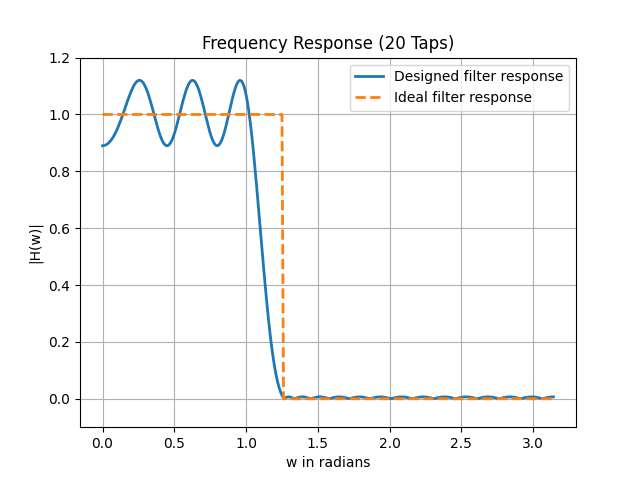
\includegraphics[width=0.7\columnwidth]{figs/A/N20_w1}
	\end{center}
\caption{$N=20$ and $\omega_c = \pi/2.5$}
\label{fig:Fig2}
\end{figure}

\begin{figure}[!h]
	\begin{center} 
	    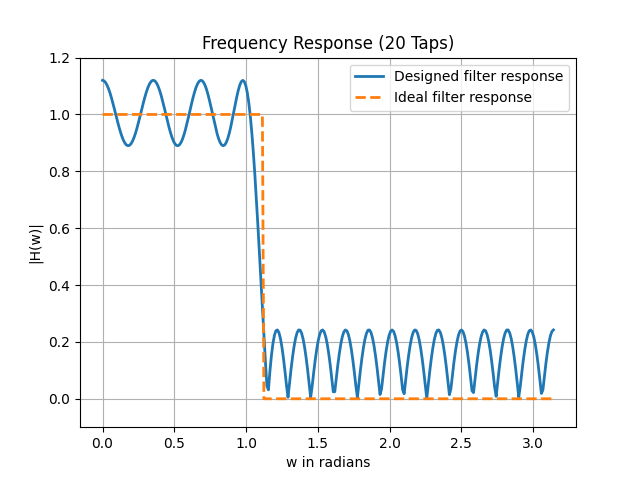
\includegraphics[width=0.7\columnwidth]{figs/A/N20_w2}
	\end{center}
\caption{$N=20$ and $\omega_c = \pi/2.8$}
\label{fig:Fig3}
\end{figure}

\begin{figure}[!h]
	\begin{center} 
	    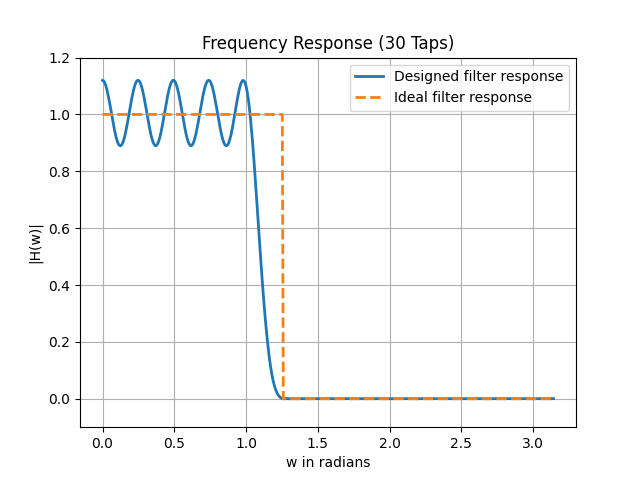
\includegraphics[width=0.7\columnwidth]{figs/A/N30_w1}
	\end{center}
%\caption{FIR filter block diagram}
\caption{$N=30$ and $\omega_c = \pi/2.5$}
\label{fig:Fig4}
\end{figure}

\begin{figure}[!h]
	\begin{center} 
	    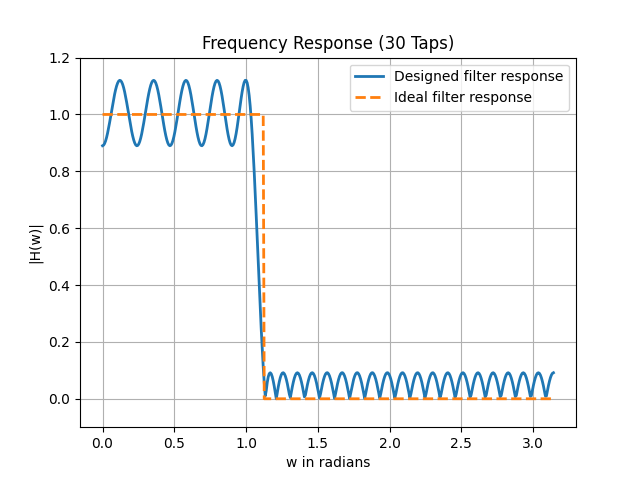
\includegraphics[width=0.7\columnwidth]{figs/A/N30_w2}
	\end{center}
%\caption{FIR filter block diagram}
\caption{$N=30$ and $\omega_c = \pi/2.8$}
\label{fig:Fig5}
\end{figure}

Deviation of the designed filter response to the ideal filter response has also been plotted as shown in figure \ref{fig:dev1}
\begin{figure}[!h]
	\begin{center} 
	    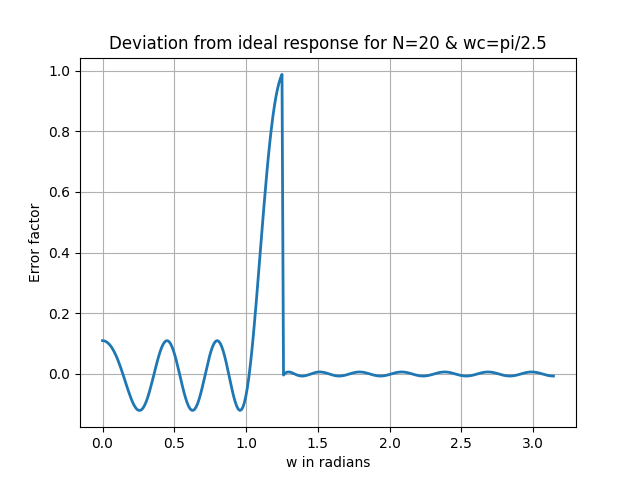
\includegraphics[width=0.7\columnwidth]{figs/dev/dev1}
	\end{center}
%\caption{FIR filter block diagram}
\caption{}
\label{fig:dev1}
\end{figure}


\item \textit{Minimum transition band}\\
Different values of $N$ and $\alpha$ have been considered, transition band is minimized. In this problem the optimal $\omega_c$ is found by linearly increasing its value from $\omega_p$ until feasibilty of the solution is obtained. The required graphs have been plotted as shown from figure \ref{fig:Fig6} to figure \ref{fig:Fig9}. 
\vspace{3mm}
\begin{center}
\begin{tabular}{ | m{3em} | m{1cm}| m{1cm}| } 
  \hline
  $\textbf{N}$& \textbf{$\alpha$}&\textbf{$\omega_c$}\\ 
  \hline
  20 & 0.006& 1.2713\\ 
  \hline
  20 & 0.08& 1.1767 \\ 
  \hline
  30 & 0.006& 1.1894 \\ 
  \hline
  30 & 0.08& 1.1264 \\ 
  \hline
\end{tabular}
\end{center}
\begin{figure}[!h]
	\begin{center} 
	    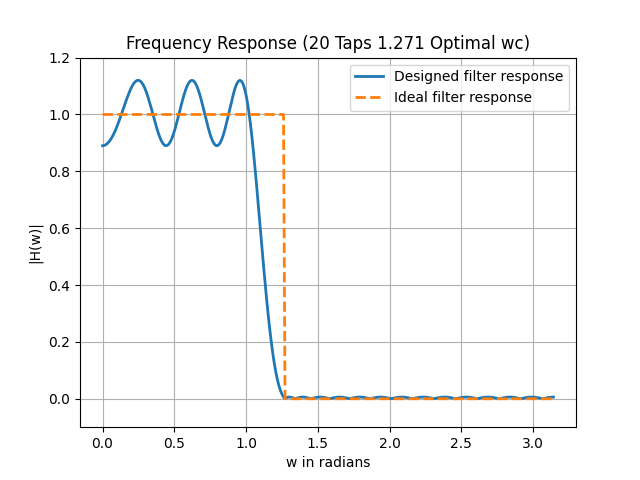
\includegraphics[width=0.7\columnwidth]{figs/B/N20_a1}
	\end{center}
%\caption{FIR filter block diagram}
\caption{$N=20$ and $\alpha = 0.006$}
\label{fig:Fig6}
\end{figure}

\begin{figure}[!h]
	\begin{center} 
	    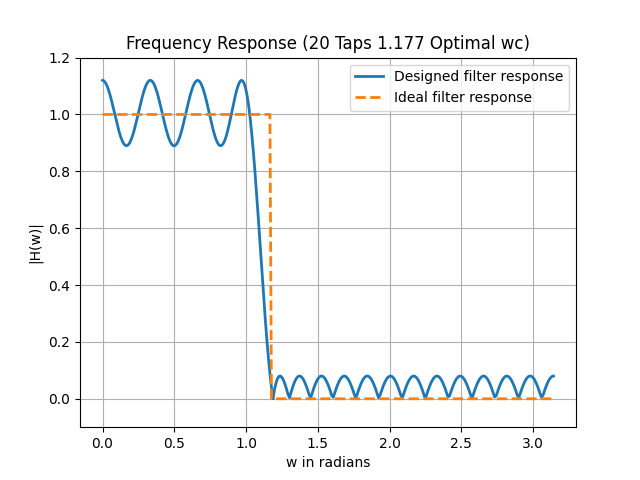
\includegraphics[width=0.7\columnwidth]{figs/B/N20_a2}
	\end{center}
%\caption{FIR filter block diagram}
\caption{$N=20$ and $\alpha = 0.08$}
\label{fig:Fig7}
\end{figure}

\begin{figure}[!h]
	\begin{center} 
	    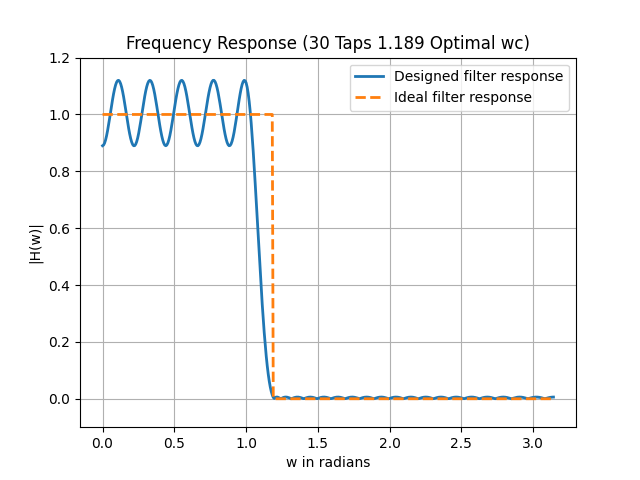
\includegraphics[width=0.7\columnwidth]{figs/B/N30_a1}
	\end{center}
%\caption{FIR filter block diagram}
\caption{$N=30$ and $\alpha = 0.006$}
\label{fig:Fig8}
\end{figure}

\begin{figure}[!h]
	\begin{center} 
	    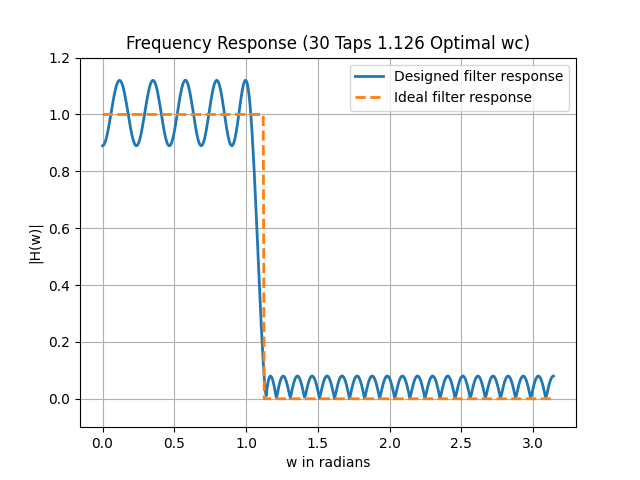
\includegraphics[width=0.7\columnwidth]{figs/B/N30_a2}
	\end{center}
%\caption{FIR filter block diagram}
\caption{$N=30$ and $\alpha = 0.08$}
\label{fig:Fig9}
\end{figure}

Deviation of the designed filter response to the ideal filter response has also been plotted as shown in figure \ref{fig:dev2}
\begin{figure}[!h]
	\begin{center} 
	    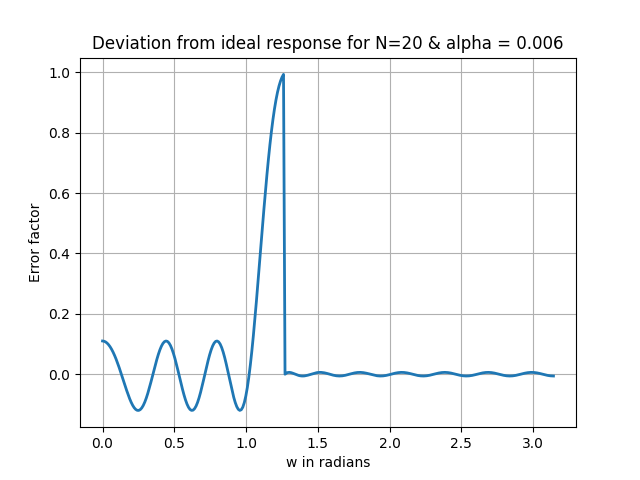
\includegraphics[width=0.7\columnwidth]{figs/dev/dev2}
	\end{center}
%\caption{FIR filter block diagram}
\caption{}
\label{fig:dev2}
\end{figure}

\newpage


\item \textit{Shortest length filter.}\\
Different values of $\omega_c$ and $\alpha$ have been considered and length of the filter $N$ is found out for each case and required graphs have been plotted. In this problem the optimal N is found by linearly increasing its value until feasibilty of the solution is obtained as shown from figure \ref{fig:Fig10} to figure \ref{fig:Fig13}.
\vspace{3mm}
\begin{center}
\begin{tabular}{ | m{3em} | m{1cm}| m{1cm} | } 
  \hline
  \textbf{$\omega_c$}& \textbf{$\alpha$} & \textbf{$N_{opt}$}\\ 
  \hline
  $pi/2.5$ & 0.006 & 21 \\ 
  \hline
  $\pi/2.5$ & 0.08 & 12 \\ 
  \hline
  $\pi/2.8$ & 0.006 & 57 \\ 
  \hline
  $\pi/2.8$ & 0.08 & 31\\ 
  \hline
\end{tabular}
\end{center}
\begin{figure}[!h]
	\begin{center} 
	    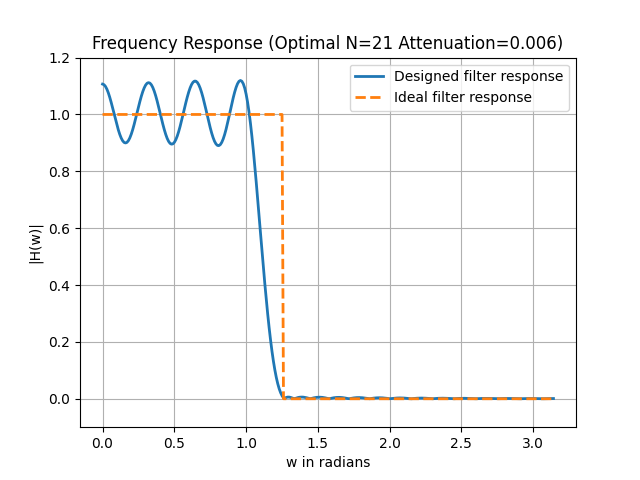
\includegraphics[width=0.7\columnwidth]{figs/C/w1_a1}
	\end{center}
%\caption{FIR filter block diagram}
\caption{$\omega_c=\pi/2.5$ and $\alpha = 0.006$}
\label{fig:Fig10}
\end{figure}

\begin{figure}[!h]
	\begin{center} 
	    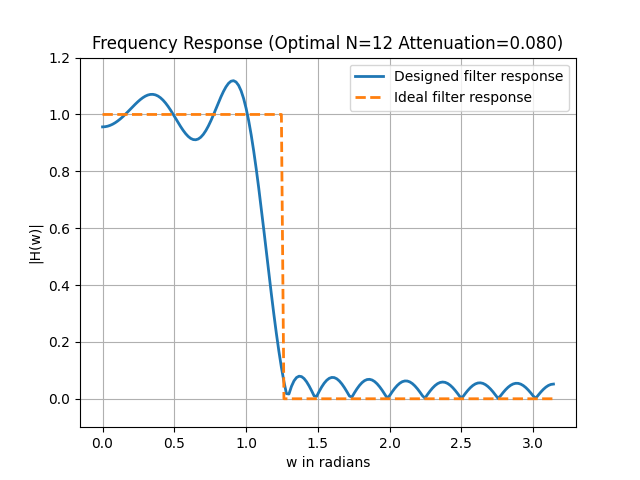
\includegraphics[width=0.7\columnwidth]{figs/C/w1_a2}
	\end{center}
%\caption{FIR filter block diagram}
\caption{$\omega_c=\pi/2.5$ and $\alpha = 0.08$}
\label{fig:Fig11}
\end{figure}

\begin{figure}[!h]
	\begin{center} 
	    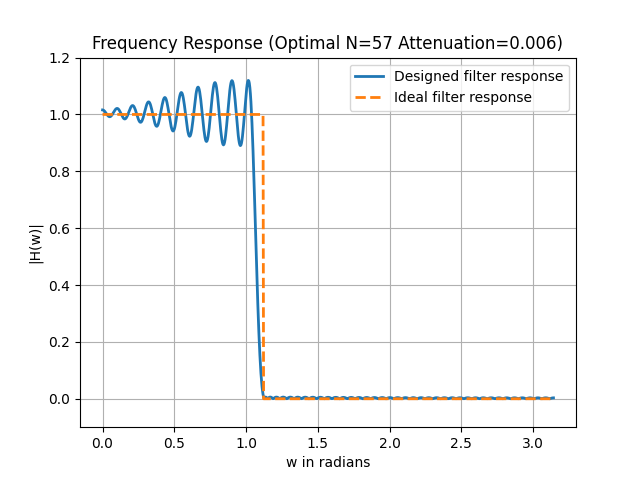
\includegraphics[width=0.7\columnwidth]{figs/C/w2_a1}
	\end{center}
%\caption{FIR filter block diagram}
\caption{$\omega_c=\pi/2.8$ and $\alpha = 0.006$}
\label{fig:Fig12}
\end{figure}

\begin{figure}[!h]
	\begin{center} 
	    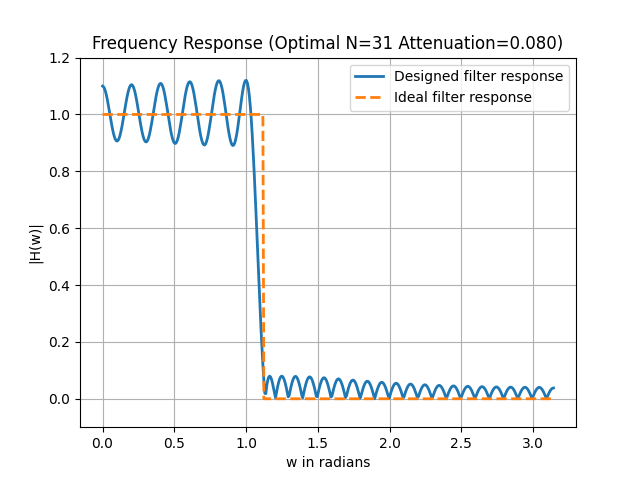
\includegraphics[width=0.7\columnwidth]{figs/C/w2_a2}
	\end{center}
%\caption{FIR filter block diagram}
\caption{$\omega_c=\pi/2.8$ and $\alpha = 0.08$}
\label{fig:Fig13}
\end{figure}
\newpage
Deviation of the designed filter response to the ideal filter response has also been plotted as shown in figure \ref{fig:dev3}
\begin{figure}[!h]
	\begin{center} 
	    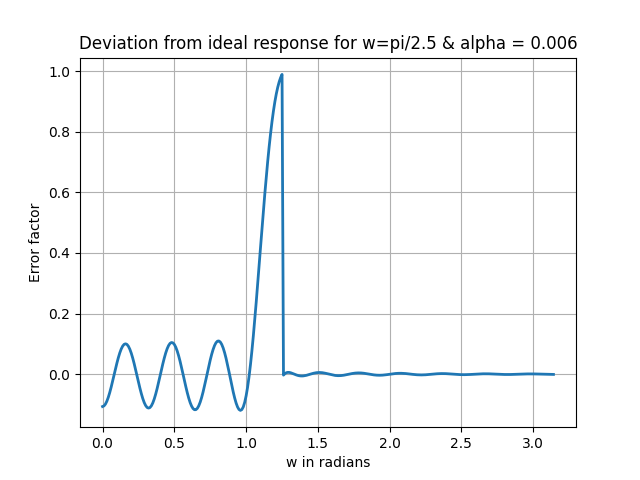
\includegraphics[width=0.7\columnwidth]{figs/dev/dev3}
	\end{center}
%\caption{FIR filter block diagram}
\caption{}
\label{fig:dev3}
\end{figure}

\end{enumerate}
\newpage

\subsection{Conclusion}
\begin{enumerate}[label=(\alph*)]
\item \textit{Maximum stopband attenuation.}\\
We observe from the plots that as the length $N$ of the filter increases, the attenuation $\alpha$ decreases and as the cutoff frequency $\omega_c$ decreases, the attenuation $\alpha$ increases.

\item \textit{Minimum transition band.}\\
We observe from the plots that as the length $N$ of the filter increases for a fixed value of $alpha$, the transition band gap decreases and keeping the length $N$ constant if we increase $\alpha$, the transition band gap decreases.

\item \textit{Shortest length filter.}\\
We observe from the plots that as cutoff frequency $\omega_c$ increases keeping $\alpha$ constant, the length $N$ of the filter increases and if we increase $\alpha$ keeping $\omega_c$ as constant, the length of filter decreases.  
\end{enumerate}

Futher this optimization problem can also be addressed throgh other complex algorithims such as spectrcal factorization, Log-Chebychev approximation and other algorithims as mentioned in the refrences below, which were not used in the current project.

\begin{thebibliography}{00}
\bibitem{b1} FIR Filter Design via Spectral Factorization and Convex Optimization by Shao-Po Wu
Stephen Boyd Lieven Vandenberghe\\ https://web.stanford.edu/~boyd/papers/pdf/magdes.pdf
\bibitem{b2} Convex Optimization – Boyd and Vandenberghe
\bibitem{b3} Stephen Boyd, Lieven Vandenberghe - Additional Exercises for Convex Optimization\\
\end{thebibliography}


















\end{document}
